\documentclass{ujarticle}
\usepackage{ketpic,ketlayer}
\usepackage{amsmath,amssymb}
\usepackage{graphicx}
\usepackage{xcolor}
\usepackage{bm,enumerate}
\usepackage[dvipdfmx,colorlinks=true,urlcolor=blue]{hyperref}

\setmargin{20}{15}{15}{15}

\西暦

\renewcommand{\labelitemi}{・}
%\pagestyle{empty}

\begin{document}

\begin{center}
KeTCindyのインストール
\end{center}

\vspace{-5mm}

\hfill 修正日:\today

\begin{enumerate}[\bf\large 1.]
\item Cinderella, R, Maxima とSumatra(Windowsのみ)をインストールする.\vspace{-2mm}

 \begin{itemize}
 \item \url{https://beta.cinderella.de}  (Cinderella)\\
\hspace*{6mm}注)Windowsの場合,右クリックして「管理者として実行」を選ぶ.
 \item \url{https://cran.r-project.org}   (R)
 \item \url{https://sourceforge.net/projects/maxima/files}  (Maxima)
 \item \url{https://www.sumatrapdfreader.org/download-free-pdf-viewer.html} (Sumatra)\\
\hspace*{6mm}注)Sumatraのインストール先は,オプションでProgram Files(またはx86)を指定する.

 \end{itemize}
\item TeXをインストールしていない場合はインストールする.\vspace{-2mm}
 \begin{enumerate}[(1)]
 \item TeXLiveを推奨 (2018以降ではketcindyが組み込まれている)
 \item KeTTeXはTeXLiveの軽量版で以下からダウンロードできる.\\
  \hspace*{10mm}\url{https://github.com/ketpic/kettex/releases}
\begin{itemize}
\item Macの場合\\
 kettex.dmgをダブルクリックして仮想ディスクを開き,KetTeX.appをApplicationsに入れる.
\item Windowの場合

\begin{enumerate}[(1)]
\item \verb|C:\|(\verb|\|は\yen の意味) に移動して解凍する.
\item \verb|kettexinst.cmd|をクリックする(詳細情報>実行)\\
・「ファイルが見つからない」のエラーは無視してよい.\\
・\verb|C:\|にkettexフォルダができる.\\
・\verb|KeTTeX-windows-20210322.zip|,\verb|KeTTeX-windows-20210322|を削除する.

\end{enumerate}
\end{itemize}
%    \hspace*{5mm}注)Mac(Catalina)の場合,ターミナルで \verb|sudo spctl --master-enable| を実行

\end{enumerate}
 
\item KeTCindyのインストール\vspace{-2mm}
  \begin{enumerate}[(1)]
  \item ketcindyをCTAN(\url{https://ctan.org})からダウンロードする.
    \begin{itemize}
     \item ketcindyで検索 $>$ Package ketcindy $>$ Download(フォルダ名はketcindy)
     \item Repositoryはgithubサイトにある最新版へのリンク\\
        \hspace*{10mm}Clone or download $>$ Download ZIP(フォルダ名はketcindy-master)\\
      \hspace*{5mm}注)Windowsでコマンドプロンプトの窓を開きたい場合,ハイフンをとってketcindymasterとする.     
     \end{itemize}
  \item \verb|ketcindysettings.cdy|をダブルクリック,以下の(1)(2)を選択して,(3)を順に実行する.
    \begin{itemize}
    \item 必要なら,実行プログラムをCinderellaに設定する.
    \item 他のcdyファイルを開いているときは,Cinderellaを一旦終了してからにする.
   \item 画面が狭ければ,右方向に広げる.
   \end{itemize}
  \end{enumerate}

%\vspace{3mm}

\begin{layer}{140}{0}
\putnotese{17}{3}{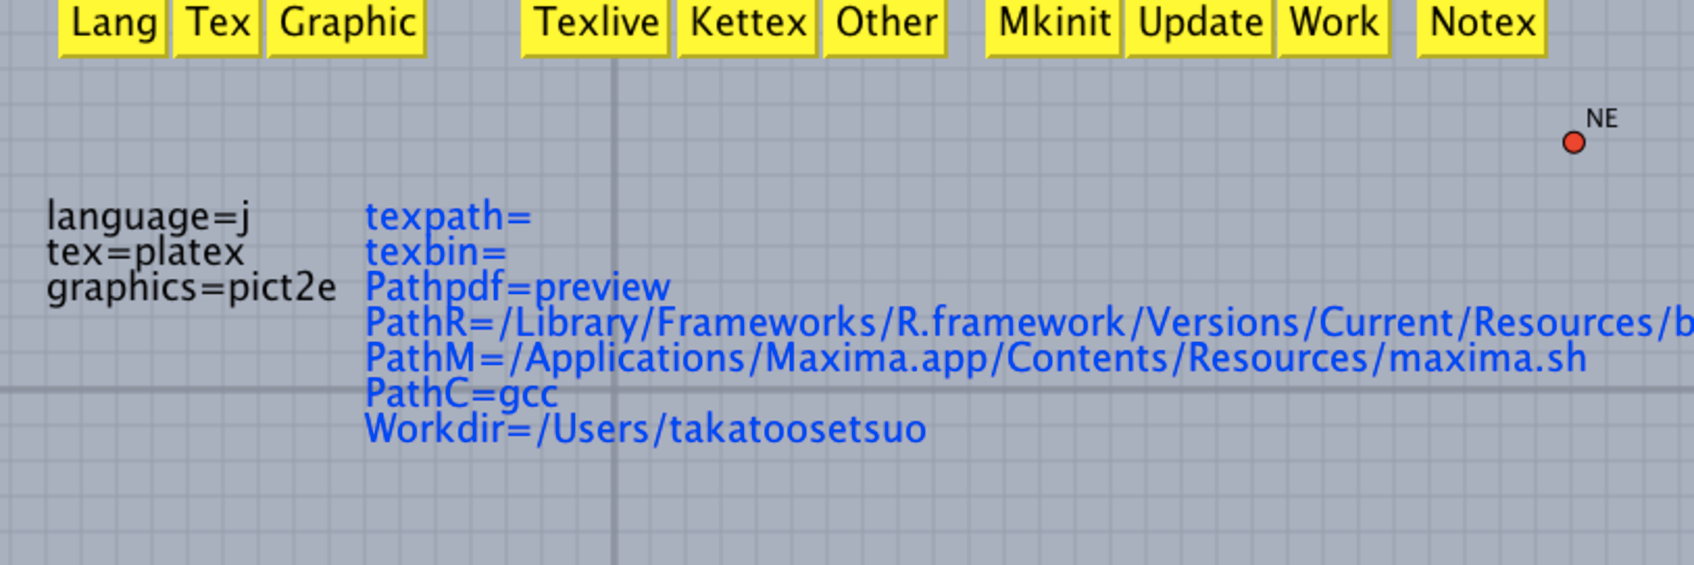
\includegraphics[bb=0.00 0.00 771.00 420.00,width=98mm]{setting.pdf}}
\putnotee{-10}{5}{\bf [1]\ 言語などの選択}
\putnotese{-7}{10}{\underline{Language}}
\putnotese{-3}{15}{Japanese, English}
\putnotese{-7}{20}{\underline{\TeX}}
\putnotese{-5}{24}{\begin{tabular}{l}
platex\\uplatex\\latex\\xelatex\\pdflatex\\lualatex\end{tabular}}
\putnotese{-7}{58}{\underline{Graphic Code}}
\putnotese{-5}{62}{\begin{tabular}{l}tpic,\ pict2e,\ tikz\end{tabular}}
\arrowline{37}{20}{20}{135}
\putnoten{63}{7}{\bf [2]\ \TeX システムの選択}
\arrowline{63}{20}{13}{90}
\putnotee{115}{5}{\bf [3]\ 作成と更新}
\arrowline{100}{20}{20}{45}
\putnotese{121}{9}{\fbox{Mkinit}}
\putnotese{123}{16}{\begin{minipage}[t]{52mm}%
初期設定ファイルketcindy.iniをユーザホーム(ホーム)に作成\\
{\small 注)CinderellaのPluginsにおくとき\\
\hspace*{3mm}CindyScript/ketlibの3行目を\\
\hfill setdirectory(plugindirectory)にする}
\end{minipage}}
\putnotese{121}{43}{\fbox{Update}}
\putnotese{123}{50}{TeXシステムのketcindyを更新}
%\putnotese{126}{56}{実行時エラーの場合Helpを参照}
\putnotese{121}{57}{\fbox{Work}}
\putnotese{123}{64}{\begin{minipage}[t]{52mm}%
作業フォルダホームに作成\\
\hfill サンプル,マニュアルなど
\end{minipage}}
\end{layer}

\vspace{70mm}

\item テストラン\vspace{-2mm}

\begin{itemize}
 \item Cinderellaをいったん終了,ketcindytestrun.cdyをダブルクリック.
\item\verb|Figure|を押して,pdfが表示されれば成功
%\item Macで「開けない」エラーが出た場合,ReadmemoreのMac版を参照.
\end{itemize}



\newpage

\item Macの補足

\begin{enumerate}[(1)]

\item TeXWorksの設定(kettexの場合)
  \begin{itemize}
  \item \url{https://github.com/TeXworks/texworks/releases/} からダウンロードできる.
  \item TeXworksを立ち上げ,「TeXworks \verb|>| 環境設定 \verb|>| タイプセット」
  \item 上の欄(パス)に\verb|kettexlive|を選択して入れる\\
  \hspace*{10mm}注) この行を上の欄の先頭に移動する.
  \item 下の欄の横にある + をクリック
    \begin{itemize}
    \item 名前:uplatex(ptex2pdf)またはplatex(ptex2pdf)
    \item プログラム : ptex2pdf
    \item 引数:\\
    \hspace*{10mm} \verb|-u|(uplatexの場合のみ)\\
    \hspace*{10mm} \verb|-l|\\
    \hspace*{10mm} \verb|-ot|\\
    \hspace*{10mm}  \verb|$synctexoption|\\
    \hspace*{10mm}  \verb|$fullname|
    \item[]OKボタンを押し,デフォルトを変更してOKボタンを押す.
    \end{itemize}
  \end{itemize}

\item TeXShopの設定(kettexの場合)
  \begin{itemize}
  \item \verb|/Applications/TeX/TexShop.app|がなければ,以下からダウンロードする.\\
  \hspace*{5mm}\url{https://pages.uoregon.edu/koch/texshop/obtaining.html}
  \item TeXShopを立ち上げ,「TeXShop \verb|>| 環境設定 |」
  \item 「書類\verb|>|設定プロファイル」 ptex(ptex2pdf)かuptex(uptex2pdf)を選ぶ
  \item 「内部設定\verb|>|パス設定」に\verb|kettex/bin/...darwin|フォルダをドラグドロップする.
  \end{itemize}

\item gccのインストール
  \begin{itemize}
    \item 曲面描画のためには, gccが必要である.
    \item Xcodeがインストールされていなければ,インストールする.\\
    \hspace*{5mm}注) ターミナルで次を実行すれば,gccだけがインストールされる.\\
    \hspace*{20mm}\verb|sudo xcode-select --install|
  \end{itemize}

\item M1でのMaximaのインストール
  \begin{enumerate}[(1)]
    \item Homebrewを以下のコマンドでインストールする.\\
 {\small \verb|/bin/bash -c "$(curl -fsSL https://raw.githubusercontent.com/Homebrew/install/HEAD/install.sh)"|}\\
  ・Homebrewを既にインストールしている場合は不要
\item Maximaをインストールする.\\
 \verb|brew install maxima|
\item \verb|type|でMaximaのインストール先を見つける(typeはMac専用).\\
 \verb|type maxima|\\
  ・\verb|/opt/local|, \verb|/usr/local|などの中にある.
\item ユーザーホームにある\verb|ketcindy.ini|のPathMに上で得たパスを入れる.
  \end{enumerate}

%\item 手動でコピーする場合(KeTTeX)\\
%\hspace*{1zw}注)他のTeXの場合は,適宜パスを置き換える.\\
%\hspace*{3zw}\verb|/Applications/kettex/texlive| $=>$ \verb|/Library/TeX/Root| など
%  \begin{enumerate}[(1)]
%  \item ketcindy(-master)/ketcindyfolderを開いておく.
%  \item scriptsフォルダの中身を以下にコピーする.\\
% \verb|/Applications/kettex/texlive/texmf-dist/scripts/ketcindy|
%  \item styleフォルダの中身を以下にコピーする.\\
% \verb|/Applications/kettex/texlive/texmf-dist/tex/latex/ketcindy|
%  \item docフォルダの中身を以下にコピーする.\\
% \verb|/Applications/kettex/texlive/texmf-dist/doc/support/ketcindy|
%  \item ターミナルで以下を実行する\\
%  \hspace*{1zw}\verb|sudo /Applications/kettex/texlive/bin/x86_64-darwin/mktexlsr|
%  \item workをユーザホームなど適当な場所にコピーして,名前(例えばketcindy)を変更する.
%  \item 上の作業ディレクトリ(ketcindy)に doc/ketmanual のマニュアルをコピーする.
%  \end{enumerate}

\item その他

\begin{itemize}
\item kettex.appの実行許可が与えられていないときは,ターミナルで\\
\hspace*{5mm}sudo xattr -r -d com.apple.quarantine    /Applications/KeTTeX.app\\
を実行する(「manなどのファイルがない」とのメッセージが出ても問題ない)
%\begin{enumerate}[(1)]
%\item ターミナルで \verb|sudo stctl --master-disable| を実行
%\item システム環境設定>セキュリティとプライバシー を開く
%\item 実行の許可が「すべてを許可」になっているかを確認する
%   \end{enumerate}
%
    \item PDFの表示後,ターミナル画面を閉じるようにする
       \begin{enumerate}[(1)]
        \item アプリケーション \verb|/| ユーティリティ \verb|/| ターミナルを開く
        \item トップメニューから\\
          \hspace*{5mm}ターミナル>環境設定 \verb|>|(プロファイル)\verb|>| シェル\\
          \hspace*{10mm}「シェルが正常に終了した場合閉じる」を選択
        \end{enumerate}
\end{itemize}

\end{enumerate}

\newpage

\item Windwosの補足

\begin{enumerate}[(1)]
\item Cinderellaのインストール
\begin{itemize}
\item \url{https://beta.cinderella.de}から「保存」でダウンロードする.
\item インストーラを右クリック「管理者として実行」を選ぶ.
\item インストール先をProgram Files(または (x86))を選ぶ.
\end{itemize}

\item Sumatraのインストール
\begin{itemize}
\item \url{https://www.sumatrapdfreader.org/download-free-pdf-viewer.html} からダウンロードする.
\item {\color{red}\verb|Option|を選び},インストール先をProgram Files(または (x86))にする.
\end{itemize}

\item TeXWorksの設定(kettexの場合)
  \begin{itemize}
  \item \url{http://www.tug.org/texworks/}からダウンロードする.
   \item TeXworksを立ち上げ,「TeXworks \verb|>| 環境設定 \verb|>| タイプセット」
  \item 上の欄(パス)に以下を追加\\
  \hspace*{5mm}\verb|C:\kettex\texlive\bin\win32|\\
  \hspace*{10mm}注) 上の行を上の欄の先頭になるように移動する.
  \item 下の欄の横にある + をクリック
    \begin{itemize}
    \item 名前:uplatex(ptex2pdf)またはplatex(ptex2pdf)
    \item プログラム : ptex2pdf
    \item 引数:\\
    \hspace*{10mm} \verb|-u|(uplatexの場合のみ)\\
    \hspace*{10mm} \verb|-l|\\
    \hspace*{10mm} \verb|-ot|\\
    \hspace*{10mm}  \verb|$synctexoption|\\
    \hspace*{10mm}  \verb|$fullname|
    \item[]OKボタンを押し,デフォルトを変更してOKボタンを押す.
    \end{itemize}
  \end{itemize}

\item MinGWのインストール
  \begin{itemize}
    \item 曲面描画のためには, gccが必要である.
    \item \url{https://sourceforge.net/projects/mingw-w64/}から,\verb|mingw-w64-install.exe|
    をダウンロードして実行
  \begin{enumerate}[(1)]
  \item Program FielesまたはProgram Files(x86)にインストールする.
  \item Architecture:Windows10が32bit版の場合\verb|i686|,64bit版の場合\verb|x86_64|を選択
\end{enumerate}

 \end{itemize}

\end{enumerate}

\end{enumerate}


\end{document}